%% TITOLO
\section{Introduzione}
\label{sec:introduzione}

%% TESTO
Dalla fine della Seconda guerra mondiale, le nascenti considerazioni strutturali e teoriche 
nella musica alla ricerca di vie al di fuori del sistema tonale (in uso in Occidente dal XVII secolo),
tanto quanto l'esigenza di introdurre nuovi paradigmi all'interno delle scienze,
hanno contribuito all'avvenire di importanti punti di incontro fra le due.

In questi cambiamenti, uno dei più importanti avanzamenti nelle scienze 
risiede nell'introduzione della
cibernetica e della teoria generale dei sistemi, che hanno conseguentemente
portato alla nascita del pensiero sistemico e del concetto di scienze della complessità.
La cibernetica in particolare, che è lo studio dei sistemi o più precisamente lo studio
dell'organizzazione dei sistemi complessi, ebbe inizio durante gli anni della seconda guerra mondiale 
e si deve al fisico e matematico Norbert Weiner.
Nel 1948 Wiener pubblicò La cibernetica; in questo libro, che ottenne grande successo,
definiva l'ambito di interesse e gli obiettivi della nuova disciplina,
inaugurando anche l'uso del nuovo termine, da lui coniato.
La cibernetica ha avuto poi un ruolo centrale nello sviluppo di molti studi scientifici, e la nascita 
di nuovi ambiti come: l'intelligenza artificiale, la teoria del caos, la teoria della catastrofe,
la teoria dei controlli, la teoria generale dei sistemi, la robotica, la psicologia,
ecc.
nella mappa di B.Castellani e L.Gerrits, possiamo visualizzare con più precisione il sorgere e l'evoluzione
di questi paradigmi scientifici.

All'inizio degli anni '60 in seno alle nascita delle scienze complesse,
l'uso di sistemi di feedback e la rilevanza dei circuiti informativi chiusi nelle strutture organizzate,
ha goduto di uno slancio popolare anche nel mondo della musica,
[* cita Sanfilippo, Valle, Feedback Systems: An Analytical Framework - CYSP 1 - Roland Kayn - 
guarda tesi PhD Sanfilippo per altri autori]

\clearpage 

\begin{figure}[!h]
    \centering
    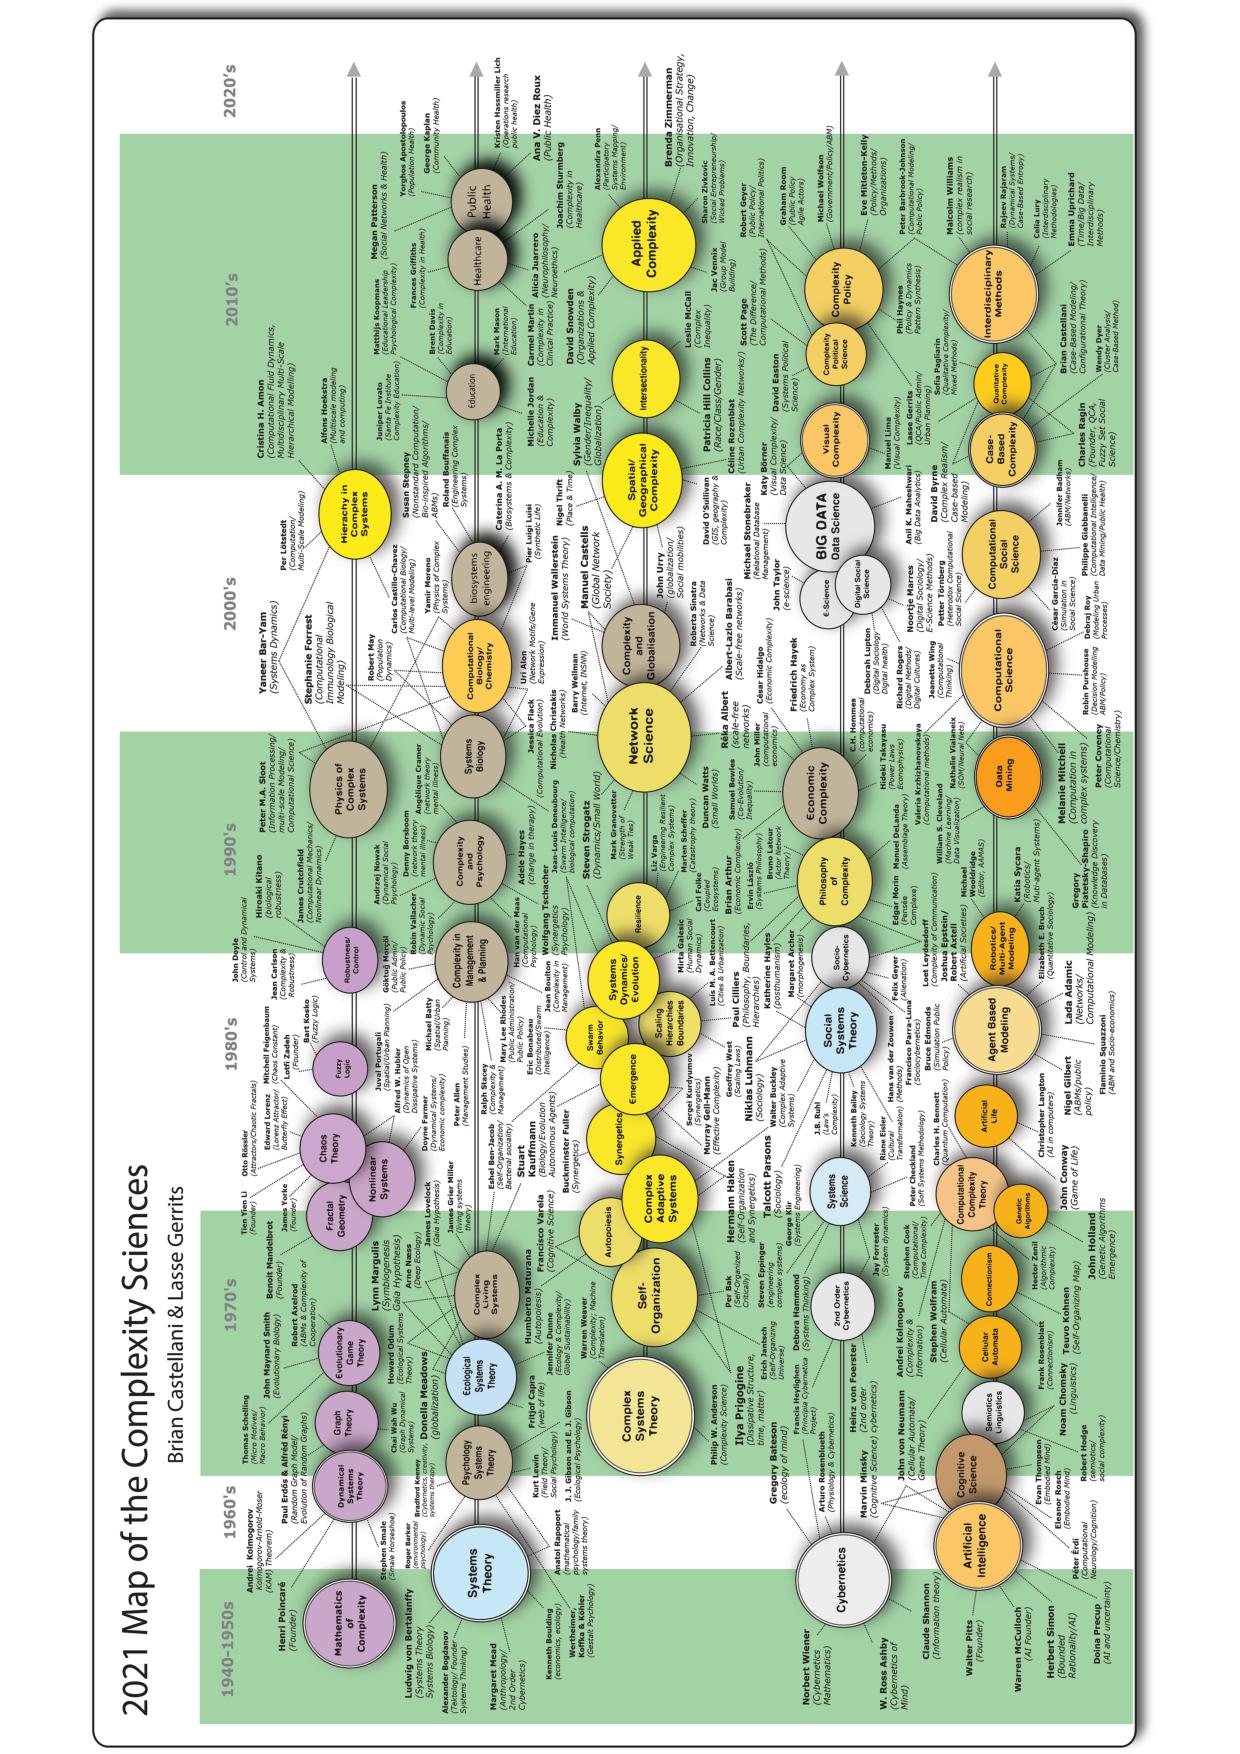
\includegraphics[width=1.0\textwidth, angle=0]{figures/complexitymap.pdf}
    \caption{B.Castellani e L.Gerrits Mappa delle Scienze Complesse}
    \label{fig:figure}
\end{figure}
%% https://www.art-sciencefactory.com/MapLegend.html

\clearpage
